\section{DTFR}
\label{sDTFR}

\hypertarget{sDTFRhy}{This}
module is used to prepare libraries for discrete-ordinates
\index{DTFR|textbf}
\index{DTF-IV}
\index{S$_{\rm N}$ transport}
transport codes that accept the format designed for the S$_{\rm N}$ code
DTF-IV\cite{DTF}.  As this was one of the early discrete-ordinats
codes, many newer S$_{\rm N}$ and
diffusion codes allow DTF format as an input option.  DTFR also
contains a simple plotting capability for providing a quick look
at its output.  DTFR was the first output module written for the
NJOY system, and it has been largely superseded by the MATXS/TRANSX
\index{MATXS/TRANSX} system.  But DTFR is still useful for some purposes
because of its simplicity.

This chapter describes the DTFR module in NJOY2016.0.

\subsection{Transport Tables}
\label{ssTTables}

Transport tables\index{transport tables} in DTF format are organized to
mirror the structure of the data inside a discrete-ordinates transport code.
\index{discrete-ordinates transport}  These codes start with the highest
energy group and work downward.  (The conventional order for group indices
is to increase as energy decreases.)  Therefore, for each group $g$, the
data required are the reaction cross sections for group $g$ and the
scattering cross sections to $g$ from other groups $g'$.  Each data element
is said to occupy a ``position'' in the table for group $g$. The
organization is shown in Table~\ref{positions}.

\begin{table}[h]
\caption{Organization of Data for One Group
  in a Transport Table}
\begin{center}
\begin{tabular}{cl}
Position & Meaning \\ \hline
  1      & edit cross sections \\
$\cdots$ &   (if any) \\
 \cword{iptotl-3}& last special edit  \\
 \cword{iptotl-2}& particle-balance absorption \\
 \cword{iptotl-1}& fission neutron production \\
 \cword{iptotl}  & total cross section \\
 \cword{iptotl}+1& upscatter $g{\leftarrow}g'\:(g'{>}g)$ \\
 $\cdots$&  (if any) \\
 \cword{ipingp}  & ingroup scattering $g{\leftarrow}g$ \\
 $\cdots$& downscatter $g{\leftarrow}g'\:(g'<g)$ \\
 \cword{itabl}   & end of table \\ \hline
\end{tabular}
\end{center}
\label{positions}
\end{table}

The basic table consists of the three standard edits, namely,
particle balance absorption ($\sigma_a$), fission neutron
production cross section ($\bar{\nu}\sigma_f$), and total cross
section ($\sigma_t$).  These standard edits are followed by the
group-to-group scattering cross sections.  If desired, the standard
edits can be preceded by \cword{iptotl-3} special edits, which can be
used in the transport code to calculate various responses of the system
(for example, heating, activation, or gas production).  If
\cword{iptotl} is the position of the total cross section, the
positions of the three standard edits will be \cword{iptotl-2},
\cword{ipingp-1}, and \cword{iptotl}, respectively.  The positions
of the special edits (if \cword{iptotl>3}) will be
1, 2, \ldots \cword{iptotl-3}.

Most transport tables describe only downscatter.  In such cases, the
position of the ingroup element is \cword{ipingp}=\cword{iptotl}+1.  Position
\cword{iptotl}+1 would contain $\sigma_{g{\leftarrow}(g{-}1)}$, and so
on.  If thermal upscatter is present, the \cword{nup} upscatter
cross sections are between the total cross section element and the
ingroup element.  Therefore, position \cword{iptotl-1} contains
$\sigma_{g{\leftarrow}(g{+}1)}$, and so on.  The position parameters
must satisfy the following conditions:
\begin{center}
     \cword{iptotl} $\ge$ 3 ~, and\\
     \cword{ipingp} = \cword{iptotl} + \cword{nup} + 1~.
\end{center}
The number of positions for a group is called the table length.
A full table will have the table length given by
\begin{center}
     \cword{itabl} = \cword{iptotl-3} + 3 + \cword{nup} + \cword{ng  ,}
\end{center}
where \cword{ng} is the total number of groups in the set.  Table
lengths can be truncated in some cases.  If this is done correctly,
the important cross sections will be conserved, and valid results
can still be obtained.

An example of a transport table is given in Table~\ref{ttable}.
This table was generated with DTFR for ENDF/B-VI $^{235}$U (\cword{mat}=9228).
It contains three special edits: the (n,2n) cross section, the fission
cross section, and the radiative capture cross section.  These are
followed by the three standard edits, and then by the ingroup
scattering for group 1.  Since this is the highest energy group,
there is no downscatter to this group from groups above, and the
rest of the positions are filled with zeros.  Group 2 starts on
line 8 with the six edit cross sections.  The seventh number is
the ingroup cross section, and the eighth is the scattering from
group 1 to group 2.  Continuing to lines 14 and 15, there are now
two downscatter elements:  two to three and one to three.
Note that there is an entire table for each Legendre order, and
that each table has a header card that describes its contents.
The ellipses were added to mark removed lines.

\newpage

\begin{table}[t]\small
\caption{Example of a Transport Table with Internal Edits}
%\begin{ccode}
\begin{verbatim}

 IL= 1 TABLE 30 GP 36 POS, MAT= 9228 IZ= 1 TEMP= 3.00000E+02
  3.2597E-01  2.0823E+00  6.1629E-04  1.3965E+00  9.7755E+00  5.9989E+00
  3.1734E+00  0.0000E+00  0.0000E+00  0.0000E+00  0.0000E+00  0.0000E+00
  0.0000E+00  0.0000E+00  0.0000E+00  0.0000E+00  0.0000E+00  0.0000E+00
  0.0000E+00  0.0000E+00  0.0000E+00  0.0000E+00  0.0000E+00  0.0000E+00
  0.0000E+00  0.0000E+00  0.0000E+00  0.0000E+00  0.0000E+00  0.0000E+00
  0.0000E+00  0.0000E+00  0.0000E+00  0.0000E+00  0.0000E+00  0.0000E+00
  4.9950E-01  2.0532E+00  1.1756E-03  1.4681E+00  9.1321E+00  5.8659E+00
  3.0495E+00  1.1523E-01  0.0000E+00  0.0000E+00  0.0000E+00  0.0000E+00
  0.0000E+00  0.0000E+00  0.0000E+00  0.0000E+00  0.0000E+00  0.0000E+00
  0.0000E+00  0.0000E+00  0.0000E+00  0.0000E+00  0.0000E+00  0.0000E+00
  0.0000E+00  0.0000E+00  0.0000E+00  0.0000E+00  0.0000E+00  0.0000E+00
  0.0000E+00  0.0000E+00  0.0000E+00  0.0000E+00  0.0000E+00  0.0000E+00
  6.8192E-01  1.8830E+00  1.5668E-03  1.1928E+00  8.0521E+00  5.7877E+00
  2.9838E+00  8.2484E-02  3.1214E-02  0.0000E+00  0.0000E+00  0.0000E+00
 ...
 IL= 2 TABLE 30 GP 36 POS, MAT= 9228 IZ= 1 TEMP= 3.00000E+02
  0.0000E+00  0.0000E+00  0.0000E+00  0.0000E+00  0.0000E+00  0.0000E+00
  2.8003E+00  0.0000E+00  0.0000E+00  0.0000E+00  0.0000E+00  0.0000E+00
  0.0000E+00  0.0000E+00  0.0000E+00  0.0000E+00  0.0000E+00  0.0000E+00
  0.0000E+00  0.0000E+00  0.0000E+00  0.0000E+00  0.0000E+00  0.0000E+00
  0.0000E+00  0.0000E+00  0.0000E+00  0.0000E+00  0.0000E+00  0.0000E+00
  0.0000E+00  0.0000E+00  0.0000E+00  0.0000E+00  0.0000E+00  0.0000E+00
  0.0000E+00  0.0000E+00  0.0000E+00  0.0000E+00  0.0000E+00  0.0000E+00
  2.5972E+00  3.8535E-02  0.0000E+00  0.0000E+00  0.0000E+00  0.0000E+00
  0.0000E+00  0.0000E+00  0.0000E+00  0.0000E+00  0.0000E+00  0.0000E+00
  0.0000E+00  0.0000E+00  0.0000E+00  0.0000E+00  0.0000E+00  0.0000E+00
  0.0000E+00  0.0000E+00  0.0000E+00  0.0000E+00  0.0000E+00  0.0000E+00
  0.0000E+00  0.0000E+00  0.0000E+00  0.0000E+00  0.0000E+00  0.0000E+00
  0.0000E+00  0.0000E+00  0.0000E+00  0.0000E+00  0.0000E+00  0.0000E+00
  2.4730E+00  2.3851E-02  7.4855E-03  0.0000E+00  0.0000E+00  0.0000E+00
 ...
 IP= 1 TABLE 30 GP 12 POS, MAT= 9228 IZ= 1 TEMP= 3.00000E+02
  0.0000E+00  0.0000E+00  1.1808E-02  2.0992E-02  2.4928E-02  5.7726E-02
  6.0219E-01  1.8328E+00  5.5365E+00  7.5176E+00  1.0018E+01  2.0404E+00
  0.0000E+00  0.0000E+00  1.0938E-02  1.9445E-02  2.4306E-02  5.8998E-02
  5.7158E-01  1.7441E+00  5.2857E+00  7.2063E+00  9.5514E+00  1.9537E+00
  0.0000E+00  0.0000E+00  8.6352E-03  1.5352E-02  2.6314E-02  7.8974E-02
  5.3190E-01  1.6485E+00  5.0937E+00  7.1114E+00  9.1307E+00  1.9158E+00
  0.0000E+00  0.0000E+00  5.0549E-03  8.9865E-03  2.9371E-02  1.0974E-01
  4.6950E-01  1.4973E+00  4.7871E+00  6.9512E+00  8.4624E+00  1.8534E+00
 ....

\end{verbatim}
%\end{ccode}
\label{ttable}
\end{table}

The last table in this example describes the photon production
matrix.  There are 30 neutron groups and 12 photon groups.  The photon
group index replaces the position index used in the neutron tables.
Therefore, the first 12 numbers in this table correspond to photon
production from neutron group 1.  The photon groups are arranged in
order of decreasing energy.

The header lines at the start of each table in this example give
the Legendre order, number of groups, number of positions,
MAT number, $\sigma_0$ number, and temperature.

DTFR will also produce a variant of the transport tables that was used
for Los Alamos libraries in years past.  These are sometimes called
``CLAW Libraries'' after the CLAW-III and CLAW-IV libraries available
from the Radiation Safety Information Computational Center (RSICC)
\index{RSICC} at the Oak Ridge National Laboratory.  Although CLAW-IV
uses a version of this format, it was actually generated using MATXS
cross sections and the TRANSX code\cite{CLAW4,TRANSX}.
\index{CLAW library!CLAW-III}
\index{CLAW library!CLAW-IV}
\index{RSICC}
\index{MATXS/TRANSX}
The key feature of the CLAW tables is that the edits are removed
from their normal position at the beginning of each group in the
transport table and written out on separate lines.  The format
specified a particular list of reactions (see Table~\ref{predef}) that
is defined using data statements in DTFR.  In addition, thermal upscatter
is not allowed in this format.  An example of this style of transport
table is given in Table~\ref{ctable}.  Note that eye-readable identifiers
were added to the right-hand edge of each card by DTFR.  The card labels
contain the first two letters of the material name, the reaction name or
the Legendre order, and a sequence number.  The format of the header
lines at the start of each table is different from the last example.
The quantity in parentheses on the ``EDIT XSEC'' card is groups by
number of edit reactions.  For the neutron tables, it is table length
by groups.  For the gamma table, it is gamma groups by neutron groups.

%\begin{table}\footnotesize
\begin{table}\small
%\begin{longtable}{cccc}
\caption{Predefined Edits for DTFR}
%\endfirsthead
%\caption{Predefined Edits for DTFR (cont.)}
%\endhead
%    \hline
%    \multicolumn{4}{r}{\emph{Continued}}
%\endfoot
%    \hline
%\endlastfoot
\label{predef}
\begin{center}
\begin{tabular}{cccc}
   Reaction Name & Position & Reaction &  Multiplicity     \\ \hline
    \cword{els} &     1   &     2    &    1  \\
    \cword{ins} &     2   &     4    &    1  \\
    \cword{n2n} &     3   &    16    &    1  \\
                &     3   &     6    &    1  \\
                &     3   &     7    &    1  \\
                &     3   &     8    &    1  \\
                &     3   &     9    &    1  \\
    \cword{n3n} &     4   &    17    &    1  \\
    \cword{ngm} &     5   &   102    &    1  \\
    \cword{nal} &     6   &   107    &    1  \\
     \cword{np} &     7   &   103    &    1  \\
   \cword{fdir} &     8   &    19    &    1  \\
    \cword{nnf} &     9   &    20    &    1  \\
   \cword{n2nf} &    10   &    21    &    1  \\
   \cword{ftot} &    11   &    18    &    1  \\
     \cword{nd} &    12   &   104    &    1  \\
     \cword{nt} &    13   &   105    &    1  \\
   \cword{nhe3} &    14   &   106    &    1  \\
    \cword{n2p} &    15   &   111    &    1  \\
    \cword{npa} &    16   &   112    &    1  \\
   \cword{nt2a} &    17   &   113    &    1  \\
   \cword{nd2a} &    18   &   114    &    1  \\
    \cword{n2a} &    19   &   108    &    1  \\
    \cword{n3a} &    20   &   109    &    1  \\
    \cword{nnd} &    21   &    32    &    1  \\
  \cword{nnd2a} &    22   &    35    &    1  \\
  \cword{nnhe3} &    23   &    34    &    1  \\
    \cword{nna} &    24   &    22    &    1  \\
   \cword{n2na} &    25   &    24    &    1  \\
   \cword{nn3a} &    26   &    23    &    1  \\
   \cword{n3na} &    27   &    25    &    1  \\
    \cword{nnp} &    28   &    28    &    1  \\
   \cword{nn2a} &    29   &    29    &    1  \\
  \cword{n2n2a} &    30   &    30    &    1  \\
    \cword{nnt} &    31   &    33    &    1  \\
  \cword{nnt2a} &    32   &    36    &    1  \\
    \cword{n4n} &    33   &    37    &    1  \\
   \cword{n3nf} &    34   &    38    &    1  \\
    \cword{chi} &    35   &   470    &    1  \\
   \cword{chid} &    36   &   471    &    1  \\
    \cword{nud} &    37   &   455    &    1  \\
    \cword{phi} &    38   &   300    &    1  \\
  \cword{theat} &    39   &   301    &    1  \\
                &    39   &   443    &    0  \\
  \cword{kerma} &    40   &   443    &    1  \\
  \cword{tdame} &    41   &   444    &    1  \\
   \cword{nusf} &    42   &     1    &    1  \\
   \cword{totl} &    43   &   452    &    1  \\ \hline
\end{tabular}
\end{center}
\end{table}
%\end{longtable}

\begin{table}\small
\caption{Example of DTFR Transport Tables Using Separate Edits}
%\begin{ccode}
\begin{verbatim}
 U235       EDIT XSEC ( 30X 48) PROC BY NJOY1  ON 05/03/90
  3.03110E+00 2.85141E+00 2.75464E+00 2.66464E+00 2.87622E+00 3.56158E+00U2  ELS
  4.43195E+00 4.38571E+00 3.94779E+00 3.53864E+00 3.34261E+00 3.61868E+00U2  ELS
  4.74566E+00 6.13164E+00 7.65700E+00 9.34710E+00 1.08466E+01 1.16438E+01U2  ELS
  1.19400E+01 1.28024E+01 1.32190E+01 1.31520E+01 1.29202E+01 1.30545E+01U2  ELS
  1.27990E+01 1.19229E+01 1.32489E+01 1.41192E+01 1.47783E+01 1.54225E+01U2  ELS
  3.78514E-01 4.17166E-01 4.61638E-01 5.44816E-01 8.11127E-01 1.37822E+00U2  INS
  2.20958E+00 2.30405E+00 2.34199E+00 2.28404E+00 2.14540E+00 1.90879E+00U2  INS
  1.60448E+00 1.29695E+00 9.63151E-01 4.00064E-01 4.54497E-02 3.03043E-03U2  INS
  1.87467E-06 7.26072E-08 0.00000E+00 0.00000E+00 0.00000E+00 0.00000E+00U2  INS
  0.00000E+00 0.00000E+00 0.00000E+00 0.00000E+00 0.00000E+00 0.00000E+00U2  INS
  3.25966E-01 4.99502E-01 6.81925E-01 8.22064E-01 6.05949E-01 3.47278E-01U2  N2N
  8.86188E-03 0.00000E+00 0.00000E+00 0.00000E+00 0.00000E+00 0.00000E+00U2  N2N
  0.00000E+00 0.00000E+00 0.00000E+00 0.00000E+00 0.00000E+00 0.00000E+00U2  N2N
  ...
 U235   L=0 N-N TABLE ( 33X 30)
  1.39646E+00 9.77549E+00 5.99892E+00 3.17345E+00 0.00000E+00 0.00000E+00U2 0
  0.00000E+00 0.00000E+00 0.00000E+00 0.00000E+00 0.00000E+00 0.00000E+00U2 0
  0.00000E+00 0.00000E+00 0.00000E+00 0.00000E+00 0.00000E+00 0.00000E+00U2 0
  0.00000E+00 0.00000E+00 0.00000E+00 0.00000E+00 0.00000E+00 0.00000E+00U2 0
  0.00000E+00 0.00000E+00 0.00000E+00 0.00000E+00 0.00000E+00 0.00000E+00U2 0
  0.00000E+00 0.00000E+00 0.00000E+00 1.46808E+00 9.13206E+00 5.86594E+00U2 0
  3.04950E+00 1.15234E-01 0.00000E+00 0.00000E+00 0.00000E+00 0.00000E+00U2 0
  0.00000E+00 0.00000E+00 0.00000E+00 0.00000E+00 0.00000E+00 0.00000E+00U2 0
  ...
 U235   L=1 N-N TABLE ( 33X 30)
  0.00000E+00 0.00000E+00 0.00000E+00 2.80033E+00 0.00000E+00 0.00000E+00U2 1
  0.00000E+00 0.00000E+00 0.00000E+00 0.00000E+00 0.00000E+00 0.00000E+00U2 1
  0.00000E+00 0.00000E+00 0.00000E+00 0.00000E+00 0.00000E+00 0.00000E+00U2 1
  0.00000E+00 0.00000E+00 0.00000E+00 0.00000E+00 0.00000E+00 0.00000E+00U2 1
  0.00000E+00 0.00000E+00 0.00000E+00 0.00000E+00 0.00000E+00 0.00000E+00U2 1
  0.00000E+00 0.00000E+00 0.00000E+00 0.00000E+00 0.00000E+00 0.00000E+00U2 1
  2.59724E+00 3.85346E-02 0.00000E+00 0.00000E+00 0.00000E+00 0.00000E+00U2 1
  0.00000E+00 0.00000E+00 0.00000E+00 0.00000E+00 0.00000E+00 0.00000E+00U2 1
  ...
 U235   L=0 N-P TABLE ( 12X 30)
  0.00000E+00 0.00000E+00 1.18077E-02 2.09916E-02 2.49277E-02 5.77264E-02U2 0
  6.02189E-01 1.83282E+00 5.53653E+00 7.51757E+00 1.00182E+01 2.04037E+00U2 0
  0.00000E+00 0.00000E+00 1.09379E-02 1.94453E-02 2.43062E-02 5.89981E-02U2 0
  5.71583E-01 1.74411E+00 5.28569E+00 7.20630E+00 9.55138E+00 1.95373E+00U2 0
  0.00000E+00 0.00000E+00 8.63521E-03 1.53515E-02 2.63136E-02 7.89737E-02U2 0
  5.31904E-01 1.64847E+00 5.09371E+00 7.11139E+00 9.13067E+00 1.91577E+00U2 0
  0.00000E+00 0.00000E+00 5.05490E-03 8.98652E-03 2.93715E-02 1.09745E-01U2 0
  ....

\end{verbatim}
%\end{ccode}
\label{ctable}
\end{table}

\subsection{Data Representations}
\label{ssDataRep}

The data stored into the transport tables are obtained from
\hyperlink{sGROUPRhy}{GROUPR}\index{GROUPR}.  Since
all the scattering matrix reactions are
kept separate in the multigroup processing, it is necessary to add
them up to compute the DTF scattering matrix.  They are obtained from
the sections with \cword{mf}=6 on the input GENDF\index{GENDF} tape.  Similarly,
all the photon production matrices have to be added up to obtain the
final DTF photon production table.  These sections have \cword{mf}=16.

\newpage
The standard edit called particle-balance absorption is used in
discrete-ordinates transport codes to calculate the balance table.
The most fundamental definition for this quantity is
\begin{equation}
   \sigma_{a,g} = \sigma_{t,g} - \displaystyle\sum_{g'}
      \sigma_{s,g'{\leftarrow}g}\,\,.
\label{abs}
\end{equation}
The total cross section is obtained from \cword{mf}=3, \cword{mt}=1
on the input GENDF
tape.  The scattering matrix is obtained by adding all the matrix
reactions found in File 6 on the input tape.  The absorption edit
is often written in the form
\begin{equation}
   \sigma_{a,g} = \sigma_{\gamma,g} + \sigma_{f,g}
         - \sigma_{n2n,g}\,\,,
\end{equation}
which is good up to the threshold for other multiparticle reactions.
Because of the presence of the (n,2n) term, the $\sigma_a$ parameter
is not equal to the real neutron absorption for high-energy groups.
In fact, it is often negative.

The next standard edit is used to compute the fission neutron
production rate when constructing a fission source.  It is used
together with a fission spectrum, which can be included in the
specials edits (see below). The fission contributions from the GENDF
tape are complicated.  First, the prompt fission matrix may be given in
\cword{mt}=18 (total fission), or in the partial fission reactions
\cword{mt}=19, \cword{mt}=20, \cword{mt}=21, and \cword{mt}=38, which
stand for (n,f), (n,n$'$f),
(n,2nf), and (n,3nf).  Second, each of these matrices may take
advantage of the fact that the shape of the fission spectrum
is constant at low energies.  Thus, fission can be represented
using single fission $\chi^{LE}_g$ vector with this shape at low energies,
with an accompanying fission neutron production cross section
$\sigma^{LE}_{Pfg}$ at low energies, and with a rectangular fission
matrix $\sigma^{HE}_{g,g{\rightarrow}g'}$ at high energies.  The
third complication is the presence of delayed fission neutron emission.
The delayed neutron yield $\bar{\nu}^D_g$ is retrieved from
\cword{mf}=3, \cword{mt}=455,
and the delayed neutron spectrum $\chi^D_g$ is obtained by adding up
the spectra for the time groups in \cword{mf}=5, \cword{mt}=455.  The following
equation shows how these separate terms are combined into the
steady-state fission neutron production edit:
\begin{equation}
   \bar{\nu}^{SS}_g\sigma_{fg}=\displaystyle
      \sum_{g'}\sigma^{HE}_{fg{\rightarrow}g'}
     +\sigma^{LE}_{Pfg} + \bar{\nu}^D_g\sigma_{fg} \,\,.
\label{ssnu}
\end{equation}
The associated steady-state fission spectrum is given by
\begin{equation}
   \chi^{SS}_{g'}= \frac{\displaystyle\sum_g\sigma^{HE}_{fg{\rightarrow}g'}
      \phi_g + \chi^{LE}_{g'}\sum_g\sigma^{LE}_{Pfg}\phi_g
       +\chi^D_{g'}\sum_g\bar{\nu}^D_g\sigma_{fg}\phi_g}
         {\rm NORM} \,\,,
\label{sschi}
\end{equation}
\vspace{1 pt}

\noindent
where NORM is the quantity that will normalize the spectrum, namely,
the sum of the numerator over all $g'$.

The total cross section is read directly from \cword{mf}=3, \cword{mt}=1.  No
transport corrections are made.  The normal convention for libraries made with
DTFR in the past was to supply P$_4$ tables and let the application
code construct transport-corrected P$_3$ tables if it wanted them.

A flexible scheme is provided for constructing special edit
cross sections.  Each position can contain any of the cross sections
available in File 3 of the GENDF tape, or a position can contain
a combination of several cross sections weighted by multiplicities.
For example, the ENDF/B-IV evaluation for $^{12}$C contains the two
reactions (n,$\alpha$) (in \cword{mf}=3, \cword{mt}=107) and (n,n$'$)3$\alpha$
(in \cword{mf}=3, \cword{mt}=91).  To obtain the helium production
cross section, it is only necessary to request an edit made up as follows:
\begin{center}
   1 $\times$ MT107 $+$ 3 $\times$ MT91~.
\end{center}

\noindent
Most of the reactions for these special edits are requested by giving
their ENDF MT numbers.  The following special MT values are used to
request some special quantities:

\begin{center}
\begin{tabular}{cl}
  Special MT & Meaning \\ \hline
     300    &  weighting flux (from \cword{mf}=3, \cword{mt}=1) \\
     455    &  delayed neutron yield (\cword{mf}=3, \cword{mt}=455) \\
     470    &  steady-state spectrum (see Eq.~\ref{sschi}) \\
     471    &  delayed neutron spectrum (\cword{mf}=5, \cword{mt}=455) \\ \hline
\end{tabular}
\end{center}
\vspace{1 pt}
See Section~\ref{ssDTFR_inp} on user input for more details.

DTFR can also construct transport tables suitable for calculations
in the thermal range.  These tables allow for upscatter, and the
user can specify that bound scattering cross sections be used in
the thermal range instead of the normal static elastic scattering
reaction.  The NJOY thermal capabilities are described in more
detail in the
\hyperlink{sTHERMRhy}{THERMR}\index{THERMR} and
\hyperlink{sGROUPRhy}{GROUPR}\index{GROUPR} sections
of this report.  In brief, NJOY can provide thermal scattering
cross sections and matrices for any material treated as a free gas in
thermal equilibrium (a Maxwell-Boltzmann distribution), or it can provide
data for a number of important moderator materials whose scattering
laws $S(\alpha,\beta)$ are available in the ENDF/B-VII libraries.
These thermal ``materials'' look like different reactions for
the dominant scattering isotope after being processed by
\hyperlink{sGROUPRhy}{GROUPR}.
Table~\ref{dtherm} lists the different binding states that are available
for ENDF/B-VII and the MT numbers used to request them.  Materials
like ``H in H$_2$O'' give the scattering for the principal scattering
isotope only; the other isotope should be treated using free-gas
scattering.  There is an exception:  benzene was evaluated as
a complete molecule, and the results were renormalized to be used
with the cross section for the dominant isotope $^{1}$H.
Therefore, this material should be used with the density
corresponding to the dominant isotope, and no thermal contribution from
the other isotope should be included at all (set both \cword{mti} and
\cword{mtc} to zero).

\begin{table}\small
\caption[Thermal Reactions Available to DTFR]{Thermal Reactions
   Available to DTFR when using the ENDF/B-VII.0 Thermal Evaluations}
\begin{center}
\begin{tabular}{ccl}
  MTI  &  MTC  &  Thermal Binding Condition \\ \hline
  221  &       &  free gas \\
  222  &       &  H in H$_2$O \\
  223  &  224  &  H in polyethylene (CH$_2$)  \\
  225  &  226  &  H in ZrH  \\
  227  &       &  Benzene \\
  228  &       &  D in D$_2$O \\
  229  &  230  &  C in graphite \\
  231  &  232  &  Be metal \\
  233  &  234  &  Be in BeO  \\
  235  &  236  &  Zr in ZrH \\
  237  &  238  &  O in BeO \\
  239  &  240  &  O in UO$_2$ \\
  241  &  242  &  U in UO$_2$ \\
  243  &  244  &  Al metal \\
  245  &  246  &  Fe metal \\ \hline
\end{tabular}
\end{center}
\label{dtherm}
\end{table}

As described in more detail in the subsection on user input, DTFR
has an input parameter called \cword{ntherm} that specifies the
number of incident-energy groups to be treated using thermal
cross sections; this parameter determines the breakpoint between
the thermal treatment and the normal static treatment.  DTFR subtracts
the static elastic cross section (\cword{mt}=2) from both the total and
absorption edits in this group range, and it adds the \cword{mti}
and \cword{mtc} cross sections to these positions.  Similarly, it
omits the contributions from the \cword{mt}=2 matrix for these
final-energy groups, and it adds in the contributions from
\cword{mti} and \cword{mtc}.  The user is free to use a number of
upscatter positions less than \cword{ntherm}.  The code will truncate
the table in a way that preserves the total thermal scattering
cross section.

\subsection{Plotting}
\label{ssDTFR_Plot}

Plots of the output data from a formatting program like DTFR are useful
in two ways: first, they provide a nice summary of the library and help
its users to understand the trends in the data easily, and second,
they are helpful in quality control as an aid to finding errors in
processing.  This versions replaces the old-style plotting from the
original version of DTFR with a nicer system making use of the NJOY
VIEWR module to produce attractive Postscript plots.

\begin{figure}[bp]\centering
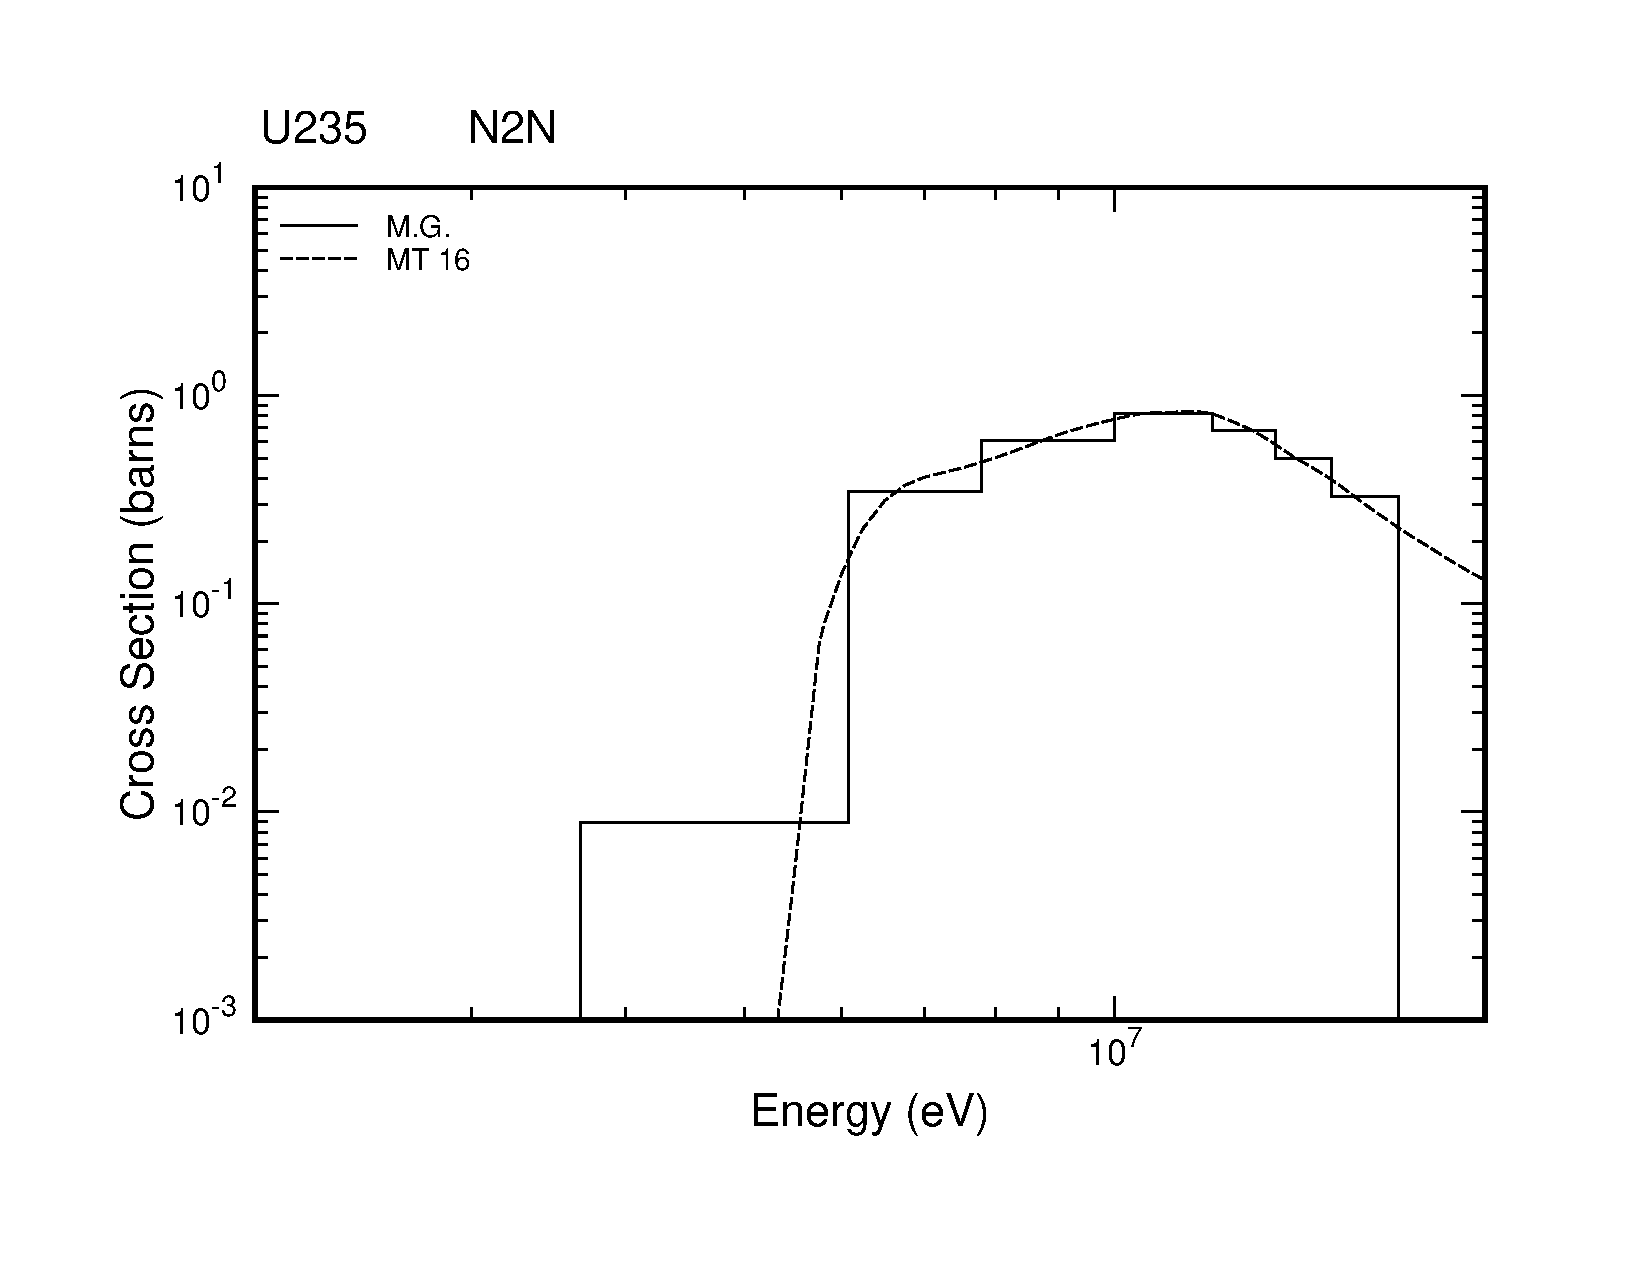
\includegraphics[keepaspectratio, height=3.0in, angle=0]{figs/dtfr1ack}
\caption[DTFR cross section plot example]{An example of DTFR plotting for
 the (n,2n) reaction of ENDF/B-VI $^{235}$U.  This plot was prepared using
 \cword{ifilm=1} and in-table edits.  All the threshold reactions are shown
 using the same energy range to make comparisons easy.}
\label{sing1}
\end{figure}

DTFR automatically makes two-dimensional log-log graphs for all the
special edit positions and the three standard edit positions.  If
available (see \cword{npend}), pointwise cross sections are plotted
on the same frame as the group cross sections.  If the multigroup
cross section is a combination of several reactions, the pointwise
cross sections for all of the components are plotted.  An example
of this will be found below.  DTFR also prepares three-dimensional
isometric projections of the P$_0$ scattering matrix and the P$_0$
photon-production table.  The user can request that one reaction
be plotted per page, or that four reactions be drawn on the same
page.  Examples of these plots are given in
Figures~\ref{sing1}--\ref{four}.

\begin{figure}[hp]\centering
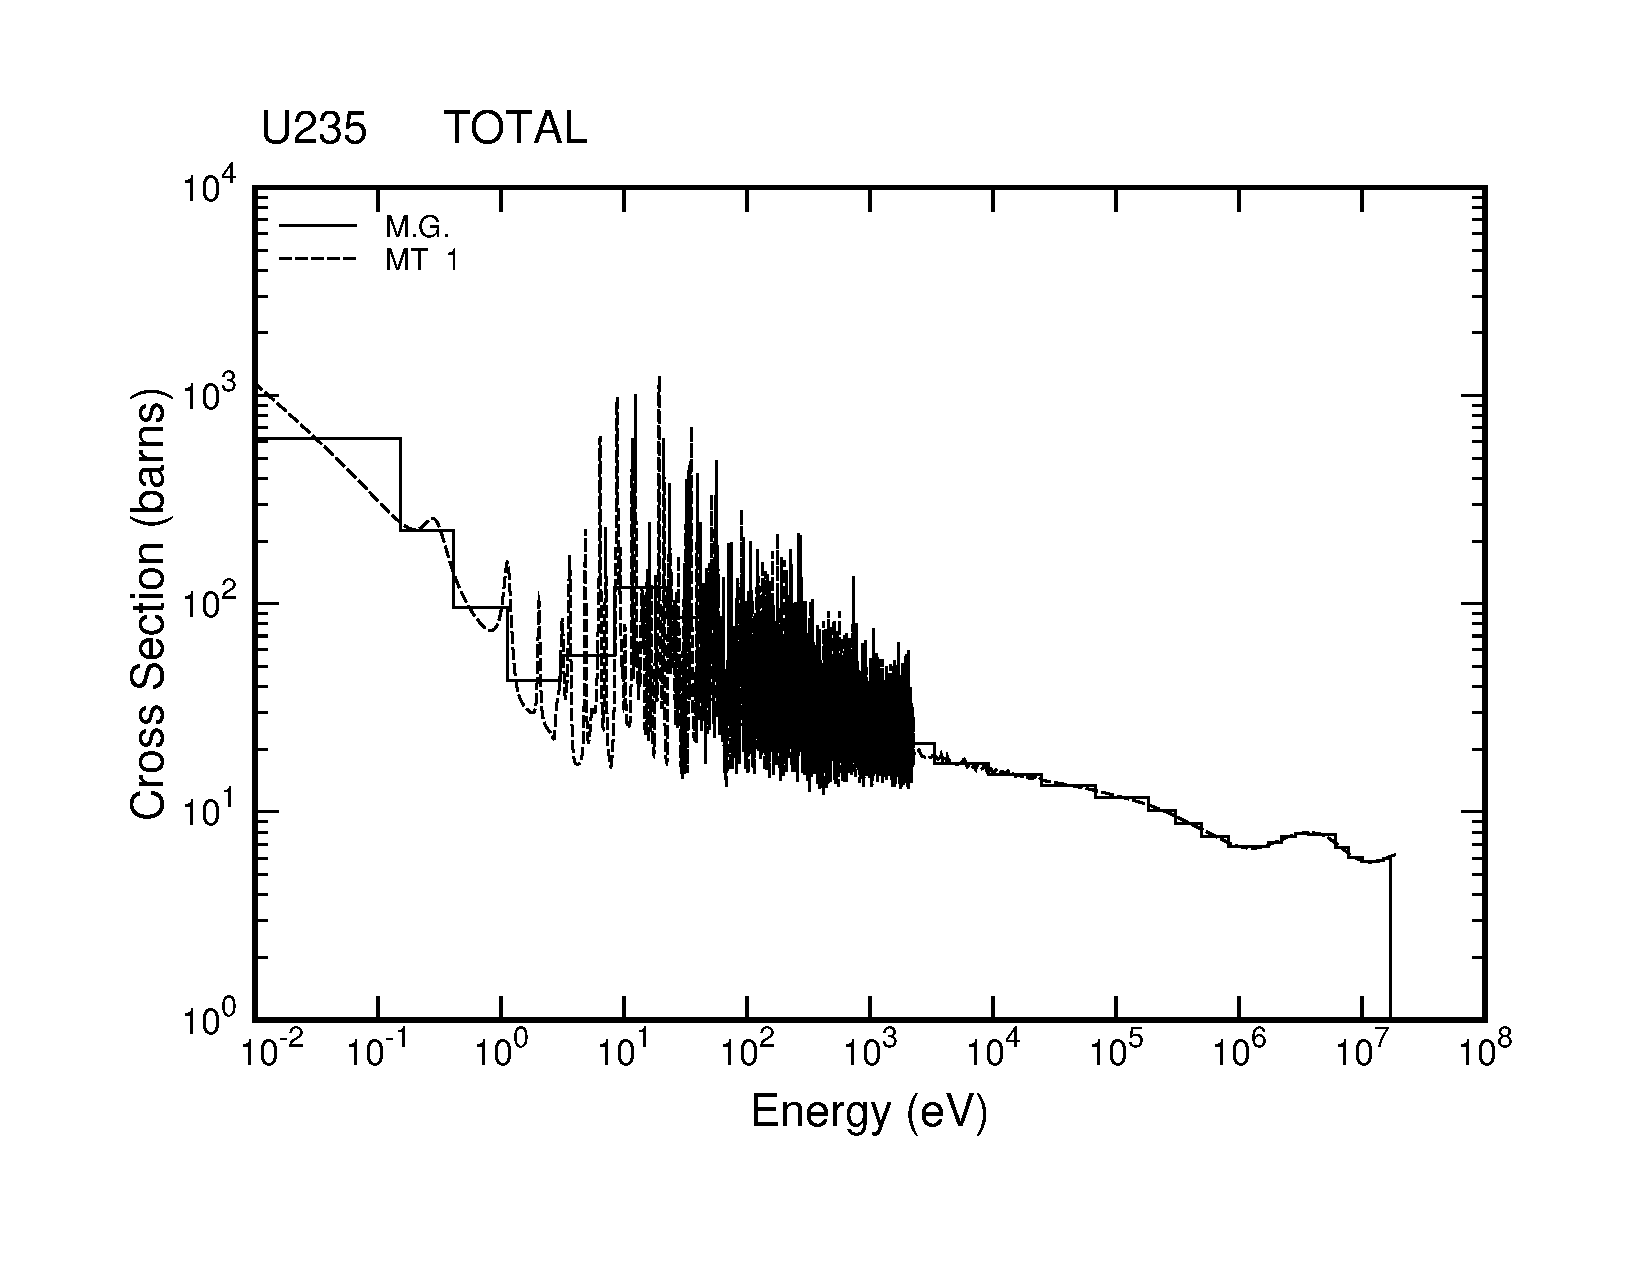
\includegraphics[keepaspectratio, height=3.2in, angle=0]{figs/dtfr2ack}
\caption[DTFR cross section plot example, expanded energy range]{This
 is the total cross section for ENDF/B-VI $^{235}$U from the same run as
 the previous plot.  The energy range from $1{\times}10^{-5}$ eV to
 $1{\times}10^{-2}$ eV was removed to expand the rest of the energy scale.}
\label{sing2}
\end{figure}

\begin{figure}[hp]\centering
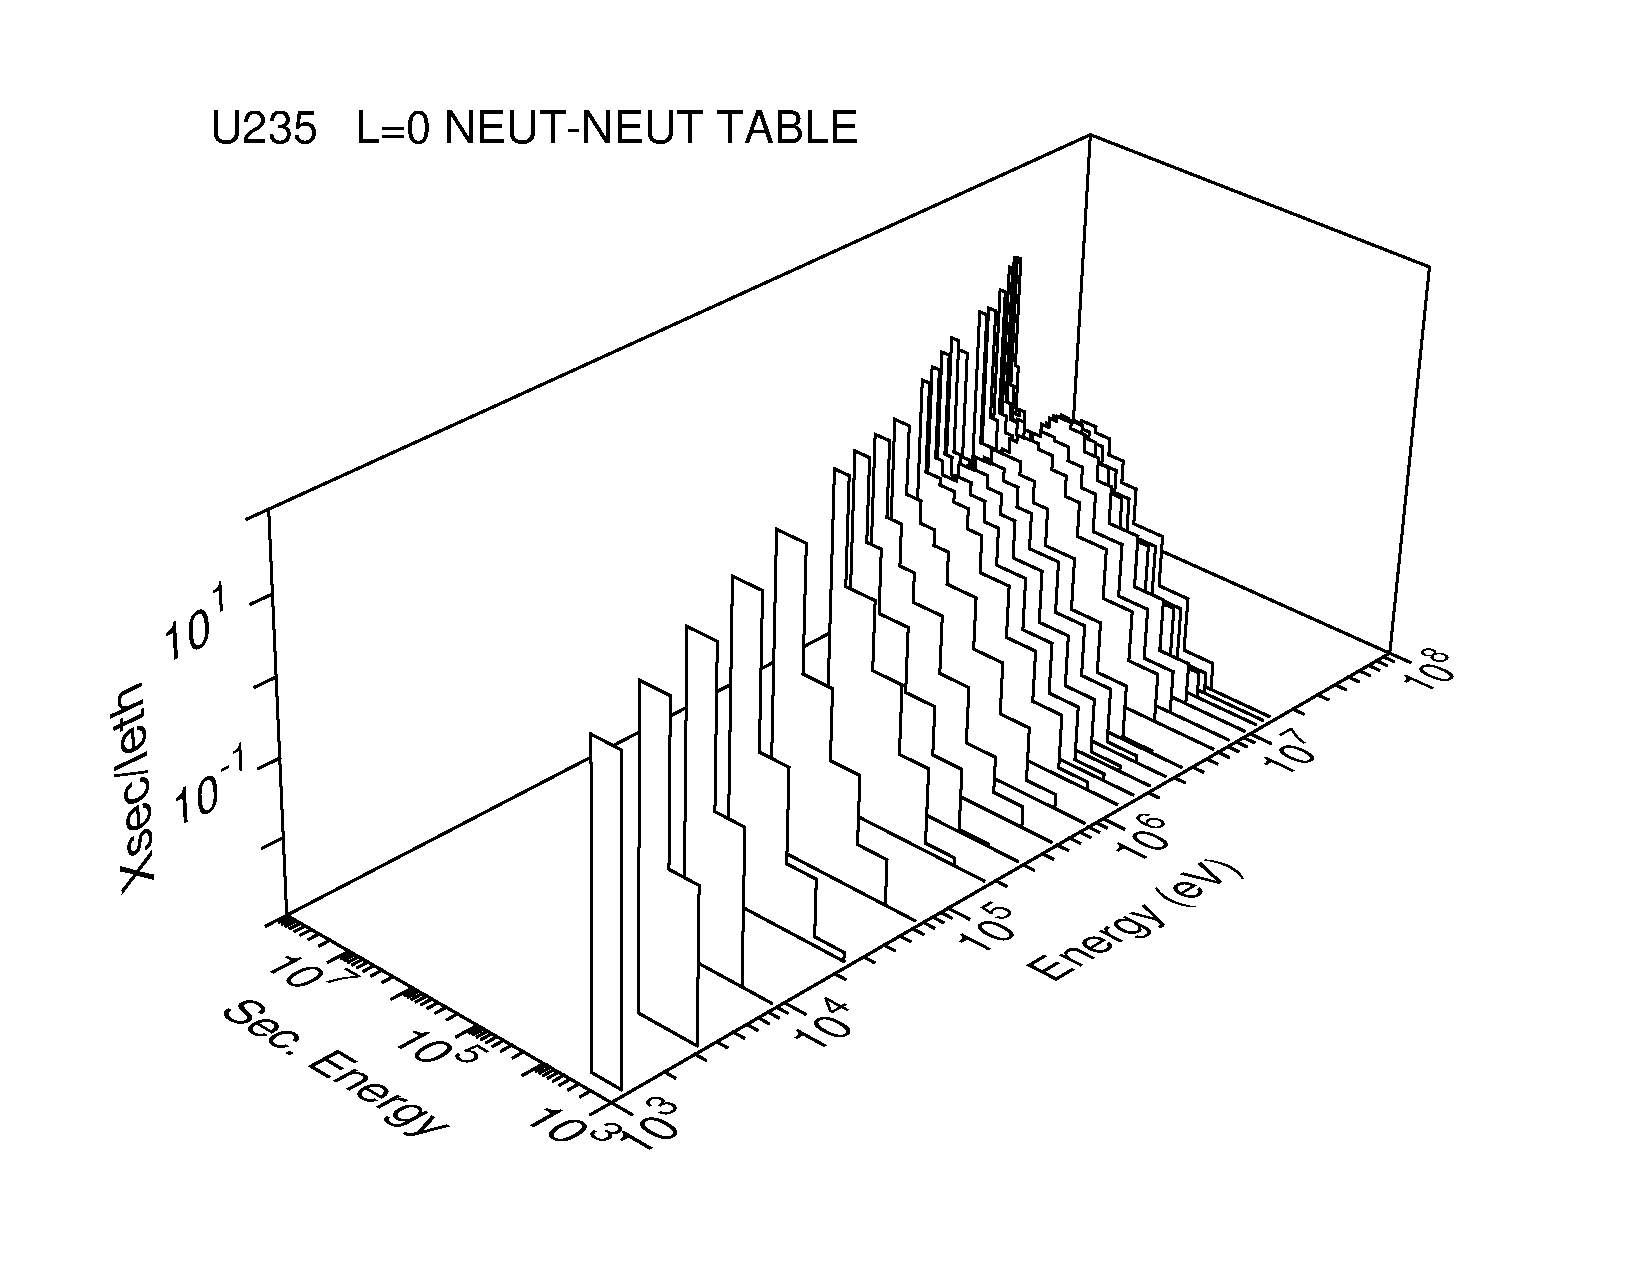
\includegraphics[keepaspectratio, height=3.2in, angle=0]{figs/dtfr3ack}
\caption[DTFR scattering matrix plot example]{This plot shows the P$_0$
 scattering matrix for ENDF/B-VI $^{235}$U by incident and secondary energy.}
\label{sing3}
\end{figure}

\begin{figure}[t]\centering
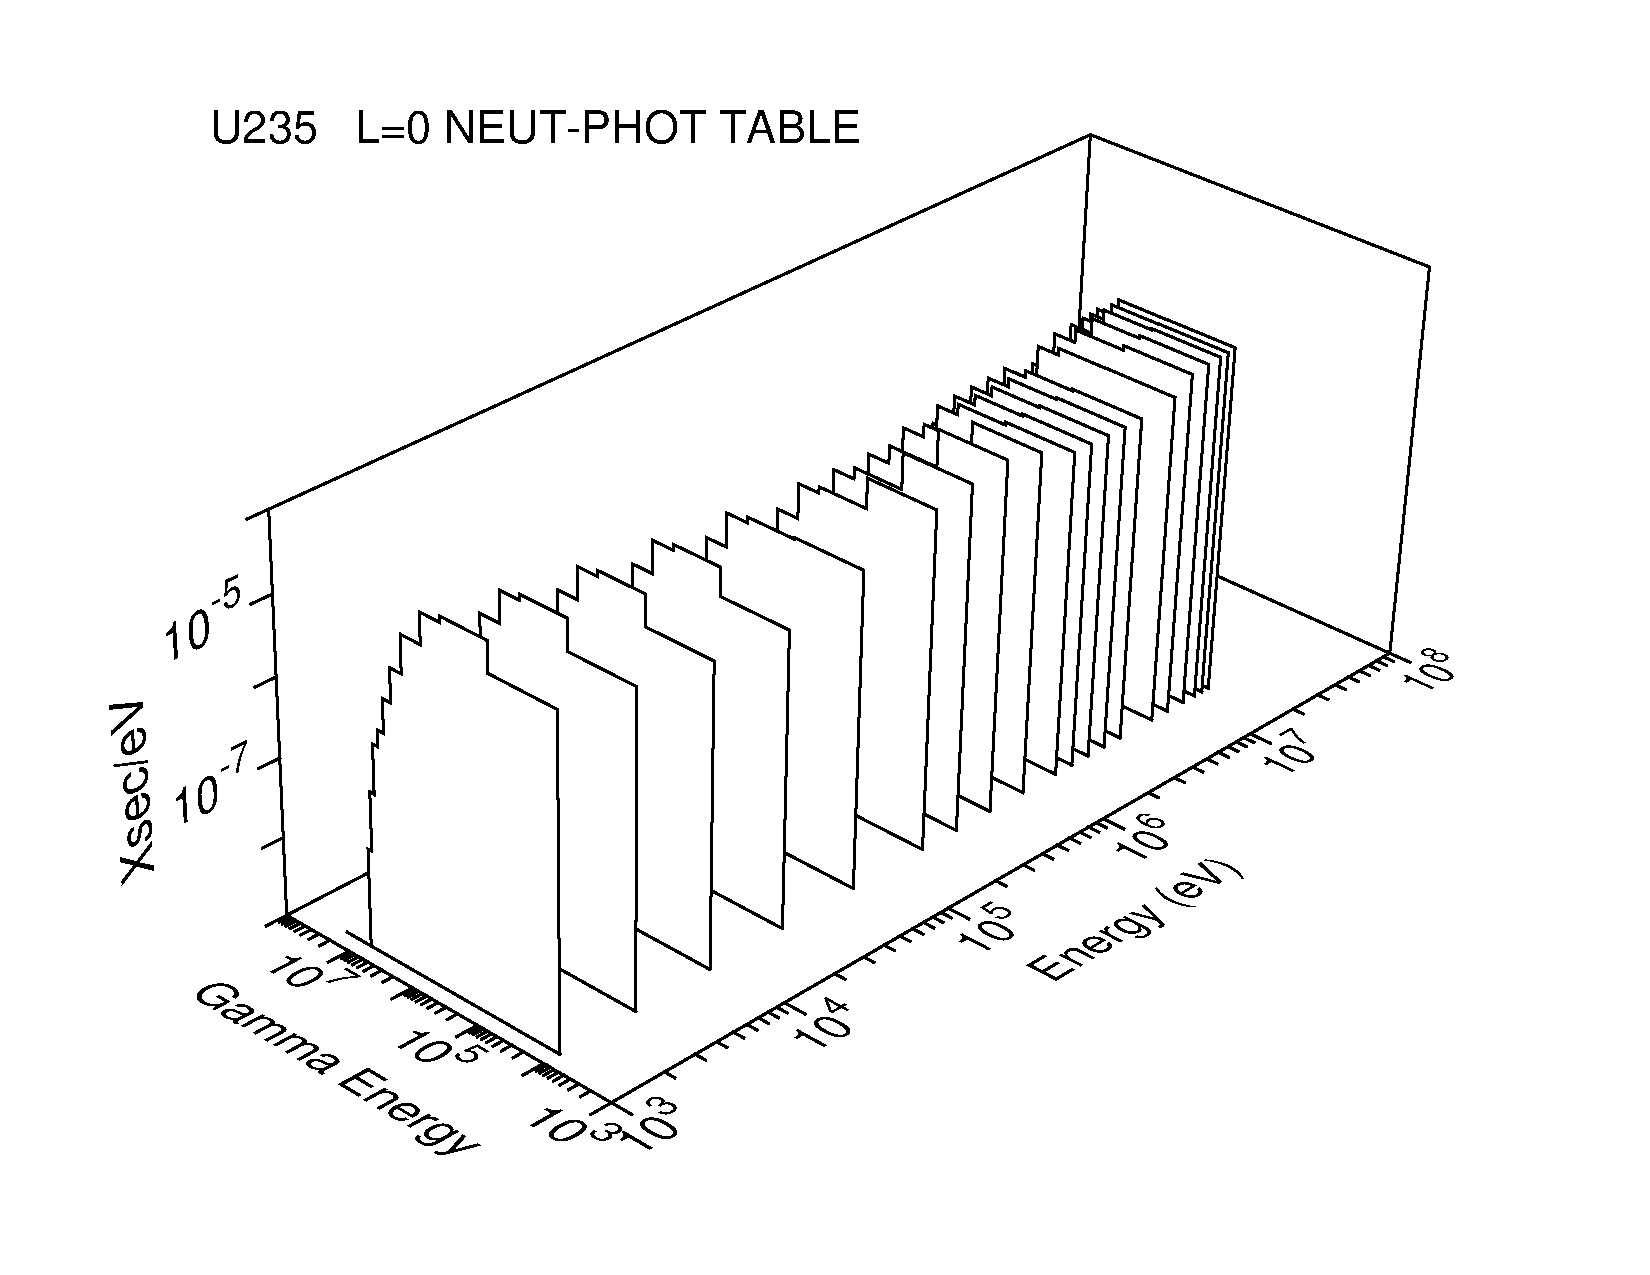
\includegraphics[keepaspectratio, height=3.2in, angle=0]{figs/dtfr4ack}
\caption[DTFR photon production matrix plot example]{The 30${\times}$12 P$_0$
 photon production matrix for $^{235}$U is plotted versus neutron energy
 and photon energy.}
\label{sing4}
\end{figure}

\begin{figure}[b]\centering
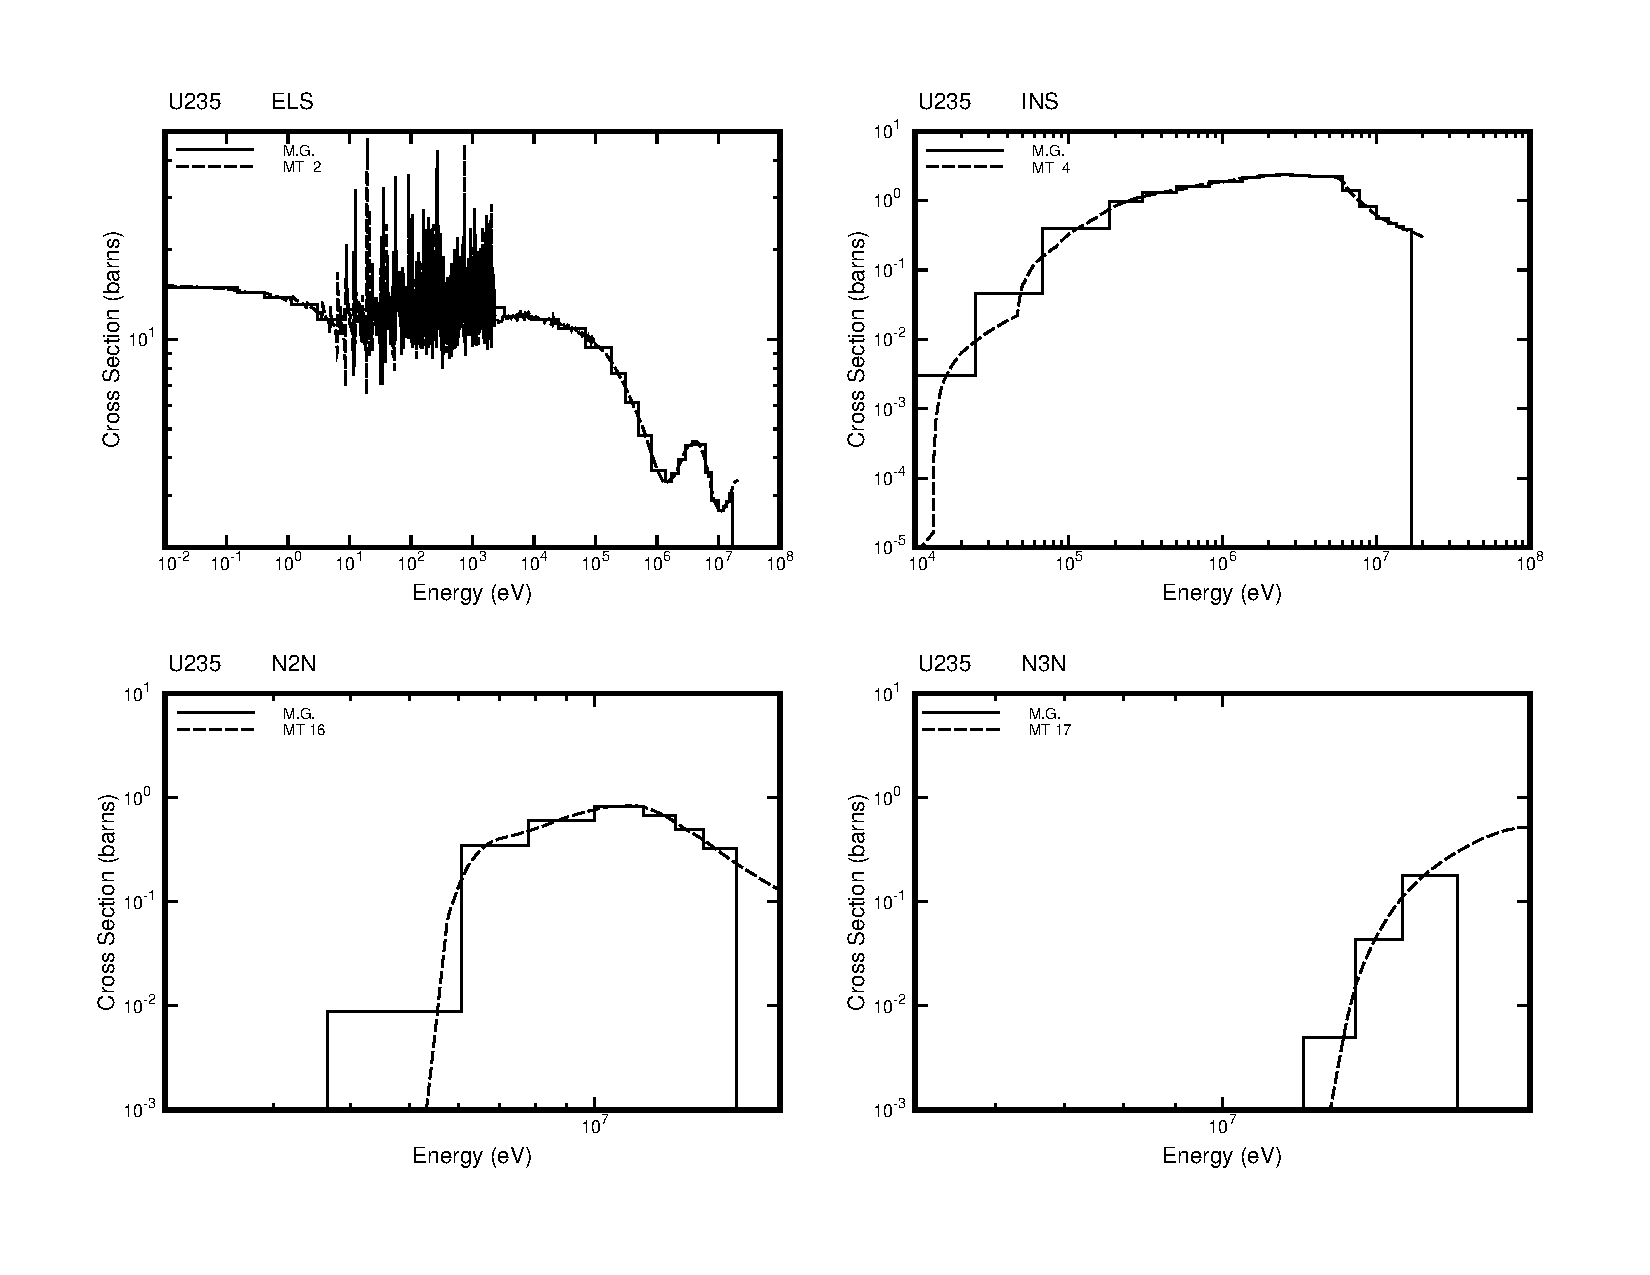
\includegraphics[keepaspectratio, height=3.2in, angle=0]{figs/dtfr5ack}
\caption[DTFR plot example, multiple plots per frame]{An example of DTFR
 plotting using \cword{ifilm=2} for ENDF/B-VI $^{235}$U for some of the
 standard edits with \cword{iedit=1}.}
\label{four}
\end{figure}

\subsection{User Input}
\label{ssDTFR_inp}

The following user input specifications were copied from the
comment cards at the beginning of the DTFR module source code.
\index{DTFR!DTFR input}
\index{input!DTFR}

\small
\begin{ccode}

   !---input specifications (free format)---------------------------
   !
   ! card 1       units
   !    nin       input unit with data from groupr.
   !    nout      output unit containing dtf tables (coded).
   !              (default=0=none)
   !    npend     input unit with pendf tape for point plots.
   !              (default=0=none)
   !    nplot     output plot info for plotr module
   !              (default=0=none)
   ! card 2       options
   !    iprint    print control (0 minimum, 1 maximum)
   !    ifilm     film control (0/1/2=no/yes with 1 plot per frame/
   !              yes with 4 plots per frame (default=0)
   !    iedit     edit control (0/1=in table/separate) (default=0)
   !
   !       cards 3 through 5 only for iedit=0
   !
   ! card 3       neutron tables
   !    nlmax     number of neutron tables desired.
   !    ng        number of neutron groups
   !    iptotl    position of total cross section
   !    ipingp    position of in-group scattering cross section.
   !    itabl     neutron table length desired.
   !    ned       number of entries in edit table (default=0).
   !    ntherm    number of thermal groups (default=0).
   !  card 3a only for ntherm ne 0
   ! card 3a      thermal incoherent and coherent mts
   !    mti       mt for thermal incoherent data
   !    mtc       mt for thermal coherent data (default=0)
   !    nlc       no. coherent legendre orders (default=0)
   ! card 4       edit names
   !       six character hollerith names for edits for as many
   !       cards as needed.  there will be iptotl-3 names read.
   !       each name is delimited with '.
   ! card 5       edit specifications
   !       ned triplets of numbers on as many cards as needed.
   !       positions can appear more than once.
   !       reaction types can appear more than once.
   !    jpos      position of edit quantity.
   !    mt        endf reaction number.
   !    mult      multiplicity to be used when adding this mt.
   !
   !       card 6 for iedit=1
   !
   ! card 6       claw-format tables
   !    nlmax     number of neutron tables (def=5)
   !    ng        number of neutron groups (def=30)
   !              (number of thermal groups is zero)
   !
   ! card 7       gamma ray tables
   !    nptabl    number of gamma tables desired (default=0)
   !    ngp       number of gamma groups (default=0)
   ! card 8       material description
   !       one card for each table set desired.
   !       empty card (/) terminates execution of dtfr.
   !    hisnam    6-character isotope name
   !    mat       material number as in endf (default=0)
   !    jsigz     index number of sigma-zero desired (default=1)
   !    dtemp     temperature desired (default=300)
   !
   !-------------------------------------------------------------------

\end{ccode}
\normalsize

As usual, card 1 is used to assign the input and output units
for the module.  \cword{nin} must be an output tape from
\hyperlink{sGROUPRhy}{GROUPR},
and it can be in either binary or coded mode.  The output
file \cword{nout} must be in coded mode.  It will contain the
DTF-format card images.  File \cword{npend} should be the same PENDF
tape that was used in \hyperlink{sGROUPRhy}{GROUPR}
when \cword{nin} was made.  It is
only needed if plots are requested.  The \cword{nplot} file will
contain the input lines that
\hyperlink{sVIEWRhy}{VIEWR} will use to prepare the Postscript
plots of the DTFR resilts.  Card 2 starts out with the print flag
\cword{iprint}, which is usually set to 1.  The parameter \cword{ifilm}
can be used to suppress plotting, or to request plots with either
1 or 4 graphs per frame.  Examples of the DTFR plotting capability
were given above.  The value of \cword{iprint} is used to control the
output format.  If it is equal to zero, a conventional DTF-type table
is produced.  If any edits were requested, they are given in the
table using the first few positions in the table.  The separate-edits
option is used to produce cross sections in the ``CLAW'' format.
In this format, the edits are extracted from the table and
written out separately with identification information appended
to the right side of each card image.  The scattering tables
have only the standard 3 edits, and they also have standard
identification fields added to the right side of each card.
Examples of both styles were given above.

Cards 3 through 5 are used for \cword{iedit=0} only.  The first
parameter is \cword{ilmax}.  It is the number of Legendre tables
desired; that is, it would be 4 for a P$_3$ set.  The number of
groups \cword{ng} must agree with the number on the input tape
from \hyperlink{sGROUPRhy}{GROUPR}.  The value of
\cword{iptotl} is used to determine both
the position of the total cross section in the table and the number
of special edit positions at the front of the table (\cword{iptotl-3},
which can be zero).  Note that \cword{ned} is not the number of
edit positions; it is the number of edit specification triplets
to be read.  Therefore, \cword{ned}$\ge$\cword{iptotl-3}.
Also \cword{ipingp}=\cword{iptotl}+1 if there is no upscatter, and
\cword{ipingp}=\cword{iptotl}+\cword{nup}+1 when the total number of upscatter
groups is \cword{nup}.  (The parameter \cword{nup} is not actually given
in the input; it is always equal to \cword{ipingp-iptotl-1}.)
The length of a full table is given by

\begin{center}
\begin{tabular}{cl}
  & \cword{iptotl-3}  \\
+ &  \cword{3}   \\
+ & \cword{nup} \\
+ & \cword{ng} \\ \hline
  & \cword{itable}
\end{tabular}
\end{center}

\noindent
However, smaller table lengths can be requested; truncation
will be performed in a way that preserves the production cross
sections.  The parameter \cword{ntherm} can be set to zero if
no thermal upscatter cross sections are desired.  If nonzero,
it refers to the number of incident thermal groups, and it is
used to define the breakpoint between the thermal and epithermal
treatments.  It is not necessarily equal to \cword{nup}.

Card 3a is only given if \cword{ntherm>0}.  It gives the \cword{mt}
numbers for the thermal incoherent and coherent cross sections to
be extracted from the GENDF tape.  Examples might include
221 and zero for free-gas scattering, or 229 and 230 for graphite.
\cword{NLC} can be used to truncate the anisotropy of the coherent
term, if desired.  For thermal cases, DTFR subtracts the
static elastic scattering from both the total and absorption
positions for the lowest \cword{ntherm} groups, and then it adds
in the cross sections corresponding to \cword{mti} and \cword{mtc}
for these thermal groups.  When reading through the matrices, it
omits all the contributions from the static elastic matrix for
the thermal groups, and adds in the \cword{mti} and \cword{mtc}
contributions for these groups instead.

Card 4 gives Hollerith names for the edit cross sections.  These
\cword{ned} names will appear on the output listing, but they
are not passed on to the output file.

Card 5 specifies the
contents of each of the special edit fields.  Note that each
edit can be any linear combination of the cross sections on the
input GENDF tape.  This feature can be used to produce complex
edits like gas production. An example follows:

\small
\begin{ccode}

  1.   ...
  2.   n.he4 kerma fiss
  3.   1 107/
  4.   1 91 3/
  5.   2 301/
  6.   3 444/
  7.   ....

\end{ccode}
\normalsize

\begin{figure}[b]\centering
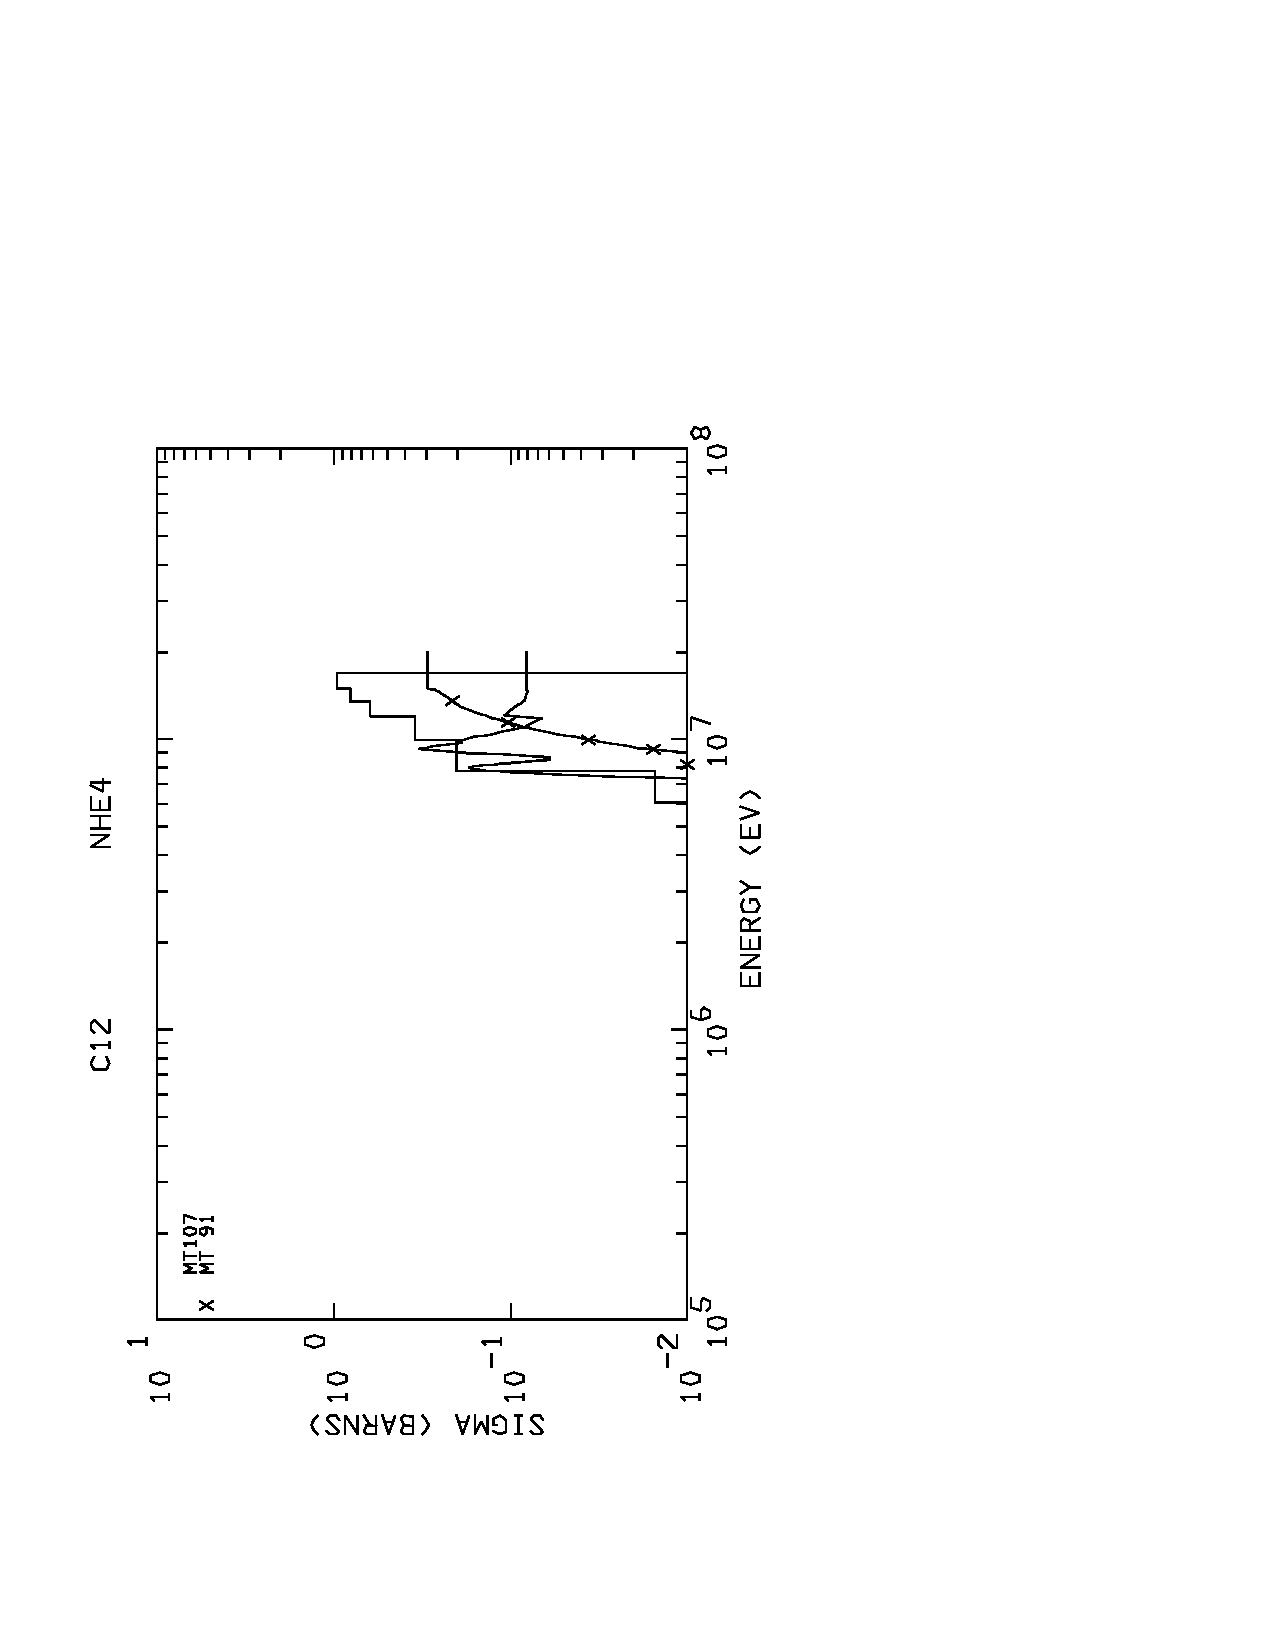
\includegraphics[keepaspectratio, height=4.0in, angle=270]{figs/dtfr6ack}
\caption[DTFR plot example, compound edit]{An example of a DTFR edit plot
   showing multiple pointwise curves that are the components
   of a compound edit.  This graph is for ENDF/B-IV $^{12}$C
   helium production.  The histogram gives the sum of the
   (n,$\alpha$) cross section and three times the
   (n,n$'$)3$\alpha$ cross section.}
\label{mult}
\end{figure}

\noindent
The line numbers are not part of the input.  Line 1 represents all
the input cards before card 4, and line 7 represents all the
cards after card 5.  This input is for ENDF/B-IV $^{12}$C.
Lines 3 and 4 construct a helium-production cross section as
the sum of (n,$\alpha$) and three times (n,n$'$)3$\alpha$.
Lines 5 and 6 assign two more edit positions for heating and
damage, respectively.  The MT numbers used for the \cword{mt}
field on card 5 are usually just the ENDF MT numbers for the
reaction.  However, there are special values available
to request the weighting flux, the steady-state and delayed
components of the fission neutron spectrum, or the delayed
fission neutron yield.  Remember that the steady-state fission
neutron production cross section will be found in position
\cword{iptotl-1} of the transport table.

When a multigroup edit is a combination of several cross sections
as in this example, the plot of the edit includes the pointwise
cross sections for all of the component reactions.  Figure~\ref{mult}
illustrates this for the $^{12}$C helium-production reaction.
Another useful technique is to build up a compound edit out of two
reactions using a multiplicity of zero for the second reaction.
This causes the second reaction to be plotted but not included in
the edit cross section.  This method can be used to compare the
energy-balance (\cword{mt}=301) and kinematic (\cword{mt}=443) versions of the
KERMA factor.  The appropriate input lines are

\small
\begin{ccode}

       ...
       heat/
       1 301 1 1 443 0/
       ...

\end{ccode}
\normalsize

\noindent
Note that this method is used in the predefined edits associated with
\cword{iedit=1} (see Table~\ref{predef}).

Card 6 is used instead if \cword{iedit=1}.  As described
above, the list of special edit cross sections is fixed for
the CLAW format.  Therefore, it is only necessary to give
\cword{nlmax} and \cword{ng}.  The number of thermal groups
is automatically set to zero.

The next card read for either choice of output format is
card 6, which controls the generation of a photon production
matrix.  The number of photon production tables is usually
zero (none), or one.  Only a few materials in the ENDF/B
libraries have anisotropic photon production data.  Of course,
\cword{ngp} must agree with the photon group structure used
in \hyperlink{sGROUPRhy}{GROUPR}.

The input deck ends with a material description card for
each material to be processed.  These materials must all be
on the input GENDF tape. (Multi-MAT GENDF tapes can be prepared
using \hyperlink{sMODERhy}{MODER} from single-material
\hyperlink{sGROUPRhy}{GROUPR} output files, but since
it is easy to combine materials at the DTF-format stage, DTFR
is usually run for one MAT at a time.) The Hollerith
material names given will appear in the comment cards before
tables and in the special labels added to the right-hand edge
of each card.  The material numbers \cword{mat} are the same ENDF
MAT numbers used when preparing the multigroup cross sections.
DTFR has only a limited capability for handling self-shielded
cross sections.  The user can specify that a given set of tables
be prepared using one particular temperature \cword{dtemp}
and one particular background cross section, the \cword{jsigz}$^{\rm{th}}$
value in the set.

\subsection{Coding Details}
\label{ssDTFR_details}

The main entry point for DTFR is \cword{dtfr}\index{dtfr@{\ty dtfr}}
from module \cword{dtfm}\index{modules!dtfm@{\ty dtfm}}, which
starts by calling \cword{ruin} to read the user's input.  Note that
the special set of edits used when \cword{iedit=1} is specified
using parameter arrays in \cword{ruin} (see \cword{kmted},
\cword{kjped}, \cword{kmultd}, and \cword{kmtid}).  The next
steps are to open a scratch file \cword{nscr} and to initialize
the plotting output.

The main loop over materials, dilution values, and temperatures
goes through statement number 105.  This is where input card number
8 is read (see input instructions) to identify the material to
be processed.  The input GENDF tape is then rewound,  and \cword{nin}
is searched for the material and temperature.  If a PENDF input tape
has been mounted, the corresponding material and temperature are
located on \cword{npend}.  Note that the materials in the input
file do not have to be in the same order as the materials on either
\cword{nin} or \cword{npend}.  If a requested material or temperature
is not found, a fatal error message is issued.

When the input files have been properly positioned, \cword{dtfr}
checks to see if there is enough storage for the tables.  The
limit \cword{nwsmax=500000} is large enough for any reasonable
multigroup set.  If larger sets are desired, increase the value of
this variable which will
automatically increase the dimension of the global array \cword{sig(nwsmax)}.
The loop over reactions and groups in a reaction goes through
statement number 150.  Once the cross sections have been read
off the input tape, the code branches to different sections to
process different kinds of data.  The first of these processes
the File 3 neutron cross sections.  Note that the total cross
section is stored in both \cword{iptotl} and \cword{iptotl-2}.  In
addition, the \hyperlink{sGROUPRhy}{GROUPR}
weighting flux can be extracted from the
section \cword{mf}=3, \cword{mt}=1 and stored into a special edit
requested using
\cword{mt}=300.  Special edit cross sections are weighted with the
specified multiplicities and summed into the specified edit
positions in the ``\cword{do ied=1,ned}'' loop.  Thermal
corrections to static scattering are made at statement number 260.
The method used is to subtract \cword{mt}=2 and add \cword{mti}
and \cword{mtc} to both the total and absorption positions.

The block of coding starting with statement number 300 is used to
accumulate the total scattering matrix.  Most numbers are simply
added into the correct position in the transport table.  The
operation specified by Eq.~\ref{abs} is performed by subtracting
all matrix elements from the absorption position.  In addition,
in the thermal range, the \cword{mti} and  \cword{mtc} data are used instead
of the \cword{mt}=2 data.

The prompt part of fission is handled starting at statement number
340.  Note that a check is made to see if MT=18 was already processed
if \cword{mt}=19 is found.  This results in a fatal error, so the user must
be careful to process only one of these representations in
\hyperlink{sGROUPRhy}{GROUPR}.
The special cases \cword{ig=0} and \cword{ig2lo=0} flag the
presence of the low-energy constant spectrum or production cross
section, respectively.  Delayed fission contributions are handled
by the next block of coding.  The method used for combining
the fission matrix, the constant-spectrum part, and the delayed
parts are defined by Eqs.~\ref{ssnu} and \ref{sschi}.  The
normalization parameter needed to fix up $\chi$ is accumulated in
the variable \cword{cnorm}.

The photon-production matrix is accumulated starting at statement
number 600.  It is a very simple process of adding all the
partial matrices with \cword{mf}=16 on the input GENDF file.
When all the reactions and groups for this material and
temperature have been processed, \cword{dtfr} calls the
subroutine \cword{dtfout}\index{dtfout@{\ty dtfout}} to prepare
the tables and plots, and then it loops back to statement number 105
for the next requested material.  After all the materials, temperatures,
and background cross sections have been written out, the plotting
system is terminated (see below), files are closed, a final
message is printed, and control is returned to \cword{njoy}.

Subroutine \cword{dtfout}\index{dtfout@{\ty dtfout}}
controls the preparation of the output DTF tables on \cword{nout},
the printing of the tables on the user's output device, and
the preparation of plots.  This is a simple routine with separate
paths for in-table edits and separate edits.  Plotting is handled
using different subroutines for the edits, the neutron table, and
the photon-production table.

Subroutine \cword{ploted}\index{ploted@{\ty ploted}} is used to
prepare plots of all the special and standard edit positions,
including overlay plots of PENDF cross sections if \cword{npend}
is available.  Subroutine \cword{histod}\index{histod@{\ty histod}}
is used to convert the multigroup values into a pointwise
cross section with steps at each of the group boundary energies;
that is, into histogram form.  Subroutine
\cword{dpend}\index{dpend@{\ty depend}} prepares the PENDF part
of the plot by thinning the original PENDF grid down to a new grid with
$x$ spacing something like the resolution of a typical screen.
In addition, it ``thickens'' reactions, if necessary, so that
there are enough points to properly follow the curve on the
final log-log plot.  Both the histogram and PENDF data arrays
are written on the the \cword{nplot} unit as simple text
commands in \hyperlink{sVIEWRhy}{VIEWR}\index{VIEWR} format.

Subroutine \cword{plotnn}\index{plotnn@{\ty plotnn}} is used to
plot an isometric view of the neutron table.  This is done by
removing the edits from the table and then writing lines to
\cword{nplot}.  Note that the energies corresponding to the groups
are used in the \hyperlink{sVIEWRhy}{VIEWR} commands, thus producing
more realistic pictures
than the older DTFR methods was able to make.  A similar process is
performed in \cword{plotnp}\index{plotp@{\ty plotp}} for the
photon-production matrix.


\subsection{Error Messages}
\label{ssDTFR_msg}

\begin{description}
\begin{singlespace}

\item[\cword{error in dtfr***number of neutron groups disagrees with...}] ~\par
   The value of \cword{ng} in the input must be consistent with
   the number of groups on the input GENDF tape.  Check the input, and
   check whether the correct tape was mounted.

\item[\cword{error in dtfr***number of gamma groups disagrees with...}] ~\par
   Same as above, except check the number of gamma groups \cword{ngp}.

\item[\cword{error in dtfr***desired temperature not on pendf}] ~\par
   Code is unable to find \cword{mat} and \cword{dtemp} on the
   input PENDF tape \cword{npend}.  Check the input information
   and check whether the correct PENDF tape was mounted.

\item[\cword{error in dtfr***not enough storage for table}] ~\par
   There is not enough space in the \cword{sig} array to construct a table
   with so many positions and groups. See the global parameter
   \cword{nwsmax=500000}.

\item[\cword{error in dtfr***not enough storage for record}] ~\par
   There is not enough space in the \cword{a} array to read in the
   data on the GENDF tape. See the global parameter \cword{nwamax=40000}.

\item[\cword{error in dtfr***mt18 already processed//mt19 not allowed}] ~\par
   Make sure that \hyperlink{sGROUPRhy}{GROUPR} processes the fission
   matrix using either \cword{mt}=18 only, or \cword{mt}=19, 20, 21,
   and 38, but not both.

\item[\cword{error in dtfr***delayed nubar required to add delayed ....}] ~\par
   The delayed neutron yield must have been processed in
   \hyperlink{sGROUPRhy}{GROUPR}
   (\cword{mfd}=3, \cword{mtd}=455), or DTFR will be unable to construct the
   steady-state fission vectors.

\item[\cword{error in ruin***iping.le.iptotl}] ~\par
   The ingroup position \cword{iping} is normally \cword{iptotl}+1,
   and it will be larger still if thermal upscatter is to be included.
   Check input card number 3.

\item[\cword{error in ruin***not enough storage for edits}] ~\par
   See the global parameter \cword{nedmax=50}.

\item[\cword{error in dpend***npts exceeds ndim}] ~\par
   The thinning/thickening process has produced too many points
   for the arrays \cword{x} and \cword{y}.  These are global
   arrays dimensioned at by the global parameter \cword{ndim=7000}.

\end{singlespace}
\end{description}

\cleardoublepage

